\chapter{Robot Motion and Observation Models}
\graphicspath{{../../img/}}

Let us define $R$ as a function of time, which gives us the orientation at time $t$. The trajectory $R(t)$ of the continuous rotation motion satisfies $R^TR(t)=I$
Let us define:

\begin{equation*}
    \frac{\partial R(t)}{\partial t} = \dot{R}(t)
\end{equation*}

We also say that:

\begin{equation*}
    \dot{R}^T(t)R(t) + R^T(t)\dot{R}(t) = 0
\end{equation*}

Since $R^T(t)\dot{R}(t)$ is skew symmetric, there exists $\omega(t)\in \R^3$, such that $R^T(t)\dot{R}(t) = \hat{\omega}(t)$.

\begin{equation*}
    R(t) = R(0)\text{exp}(t\hat{\omega})
\end{equation*}

\begin{figure}[h]\centering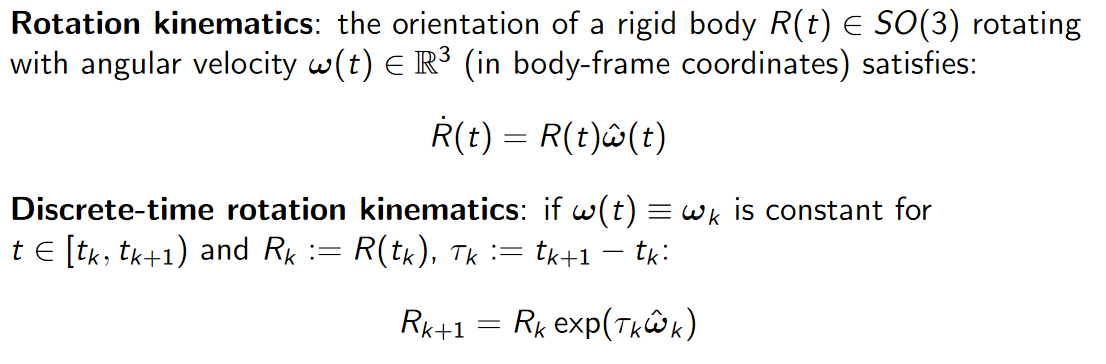
\includegraphics[width=10cm]{img/j_4_1.png}\end{figure}

We can do the same thing with quaternions:

\begin{figure}[h]\centering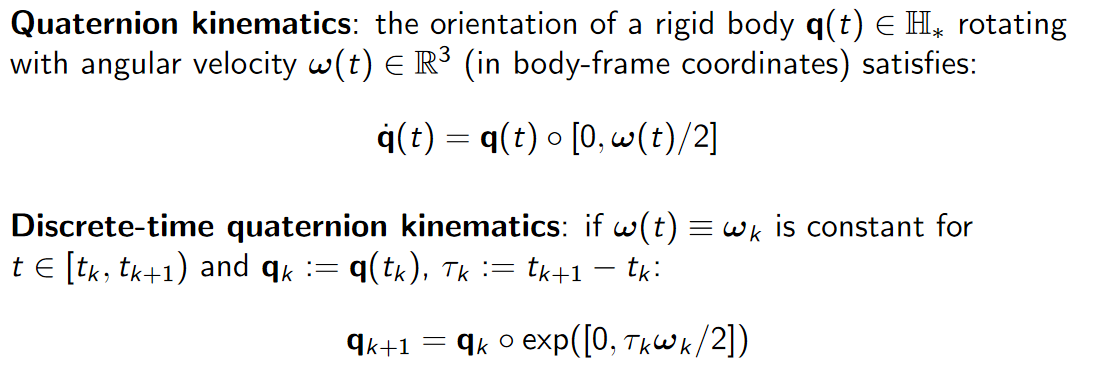
\includegraphics[width=12cm]{img/j_4_2.png}\end{figure}

To represent this for a general pose, we must consider the linear velocity and angular velocity, which is also called twist.

\begin{figure}[h]\centering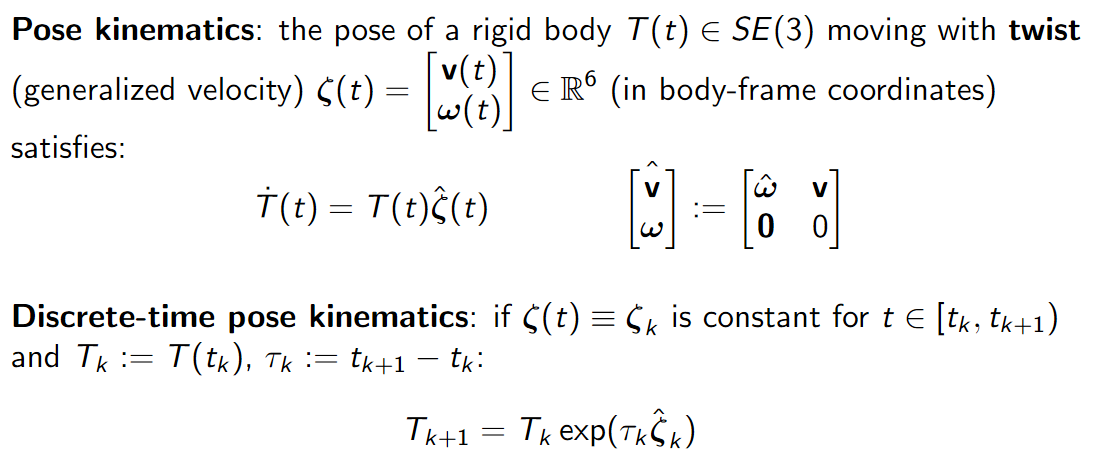
\includegraphics[width=12cm]{img/j_4_3.png}\end{figure}

If there are forces acting on the pose (we may not use this in the course), then it's called pose dynamics.

\begin{figure}[h]\centering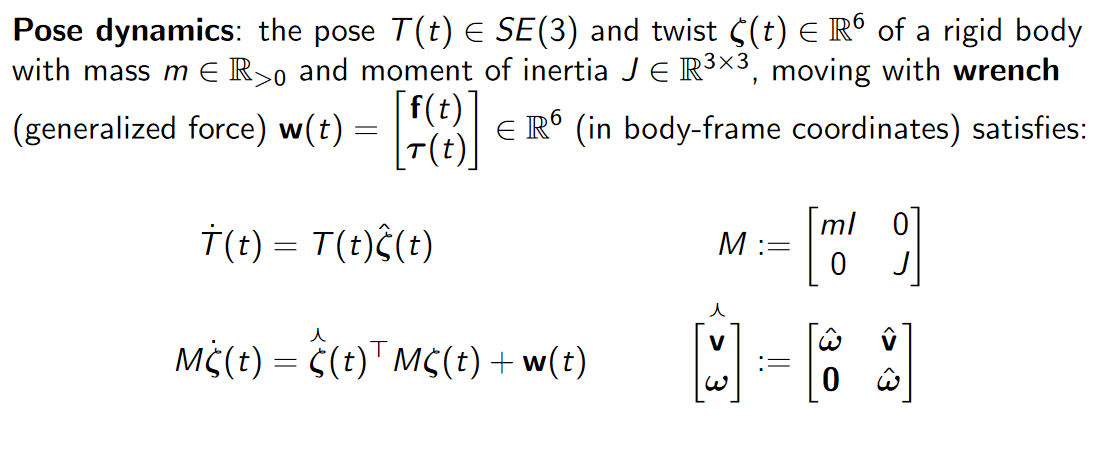
\includegraphics[width=10cm]{img/j_4_4.png}\end{figure}

Here $\textbf{f}$ is the force, and $\tau$ is the torque.

\section{Motion Models}

\begin{figure}[h]\centering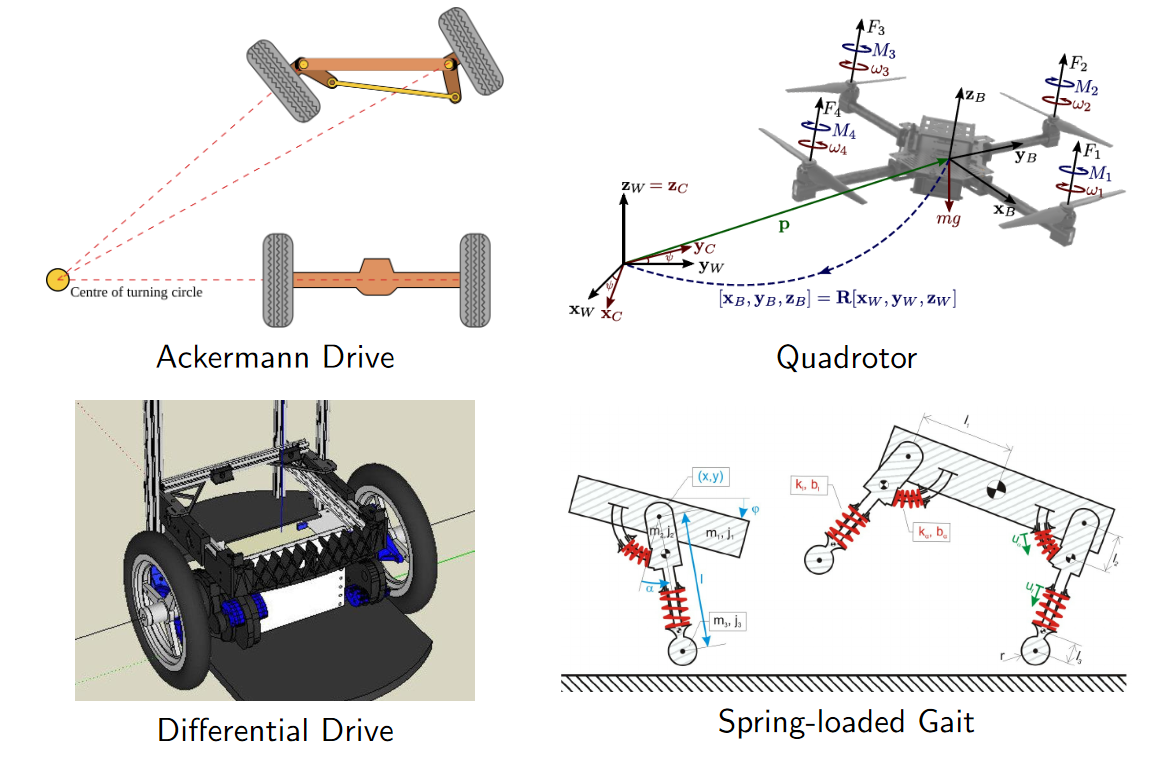
\includegraphics[width=12cm]{img/j_4_5.png}\end{figure}

We will consider the ackerman and differentiable drive robots primarily.

There are a few variables describing the robot system:

\begin{enumerate}
    \item time $t$
    \item state $x$ (position, orientation)
    \item control input $u$ (velocity, force)
    \item disturbace $w$ (tire slip, wind)
\end{enumerate}

A motion model is a function $f$ relating the current state $\x$ and input $\u$ of a robot with its state change:

\begin{itemize}
    \item Continuous: $\dot{\x}(t) = f(\x(t), \u(t))$
    \item Discrete: $\x_{t+1} = f(\x_t, \u_t)$
\end{itemize}

\begin{figure}[h]\centering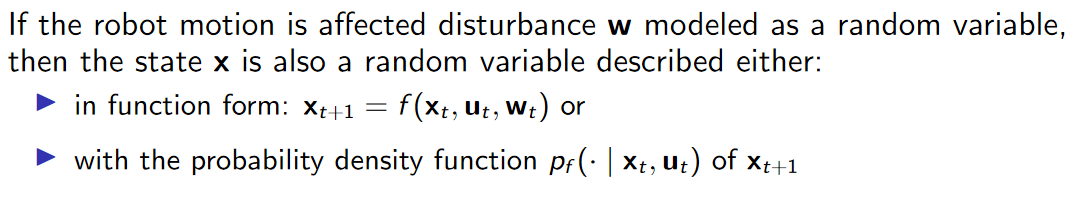
\includegraphics[width=12cm]{img/j_4_6.png}\end{figure}

\section{Odometry}

Consider a rigid-body robot with state $\x_t = T_t \in SE (3)$ capturing the robot pose in the world frame $\{W \}$ at time $t$.

Determining the change of pose using sensors on the robot is known as odometry, which is done using onboard sensors.

\begin{figure}[h]\centering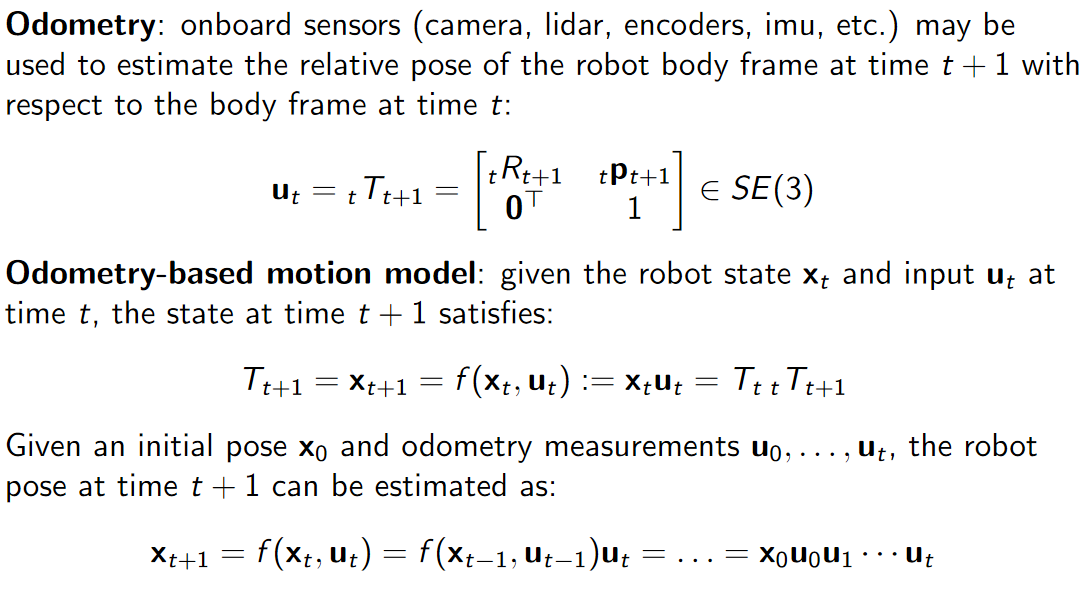
\includegraphics[width=12cm]{img/j_4_7.png}\end{figure}

The odometry estimate will drift however over time, because small measurements errors in each $\u$ will accumulate.

Now, if our state $X_k = T_k$, is given an input $u_k$, which is the twist $\left(\begin{bmatrix}v_k\\ \omega_k\end{bmatrix}\right)$.

Now, we can compute the new pose using:

\begin{figure}[h]\centering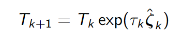
\includegraphics[width=5cm]{img/j_4_8.png}\end{figure}

Where teh fancy symbol is the twist, $\tau$ is the $t_{k+1}-t_k$.

\section{Differential-Drive Kinemantic Model}

This robot cannot move sideways - or its degrees of freedom are limited - so it is a non-holonomic robot. 

\begin{figure}[h]\centering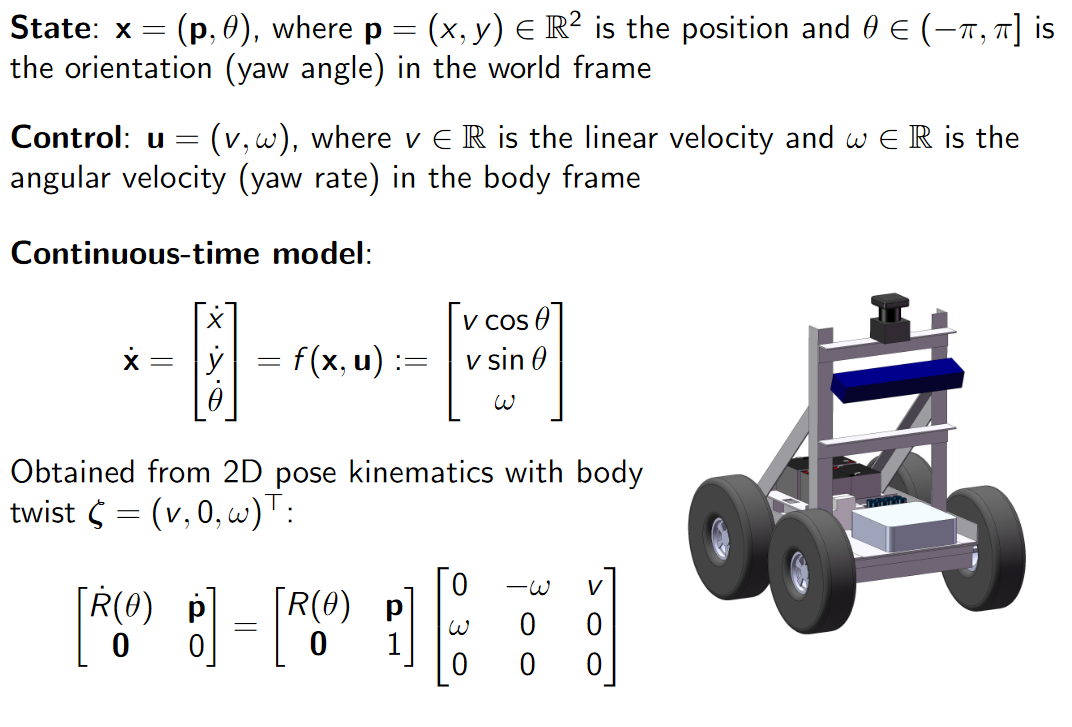
\includegraphics[width=12cm]{img/j_4_9.png}\end{figure}

We can make a discrete version of this using euler discretization. This means that we approximate our derivative $\dot{s} = \frac{s_{k+1}-s{k}}{\tau_k}$. There is also an exact integration that is possible.


\begin{figure}[h]\centering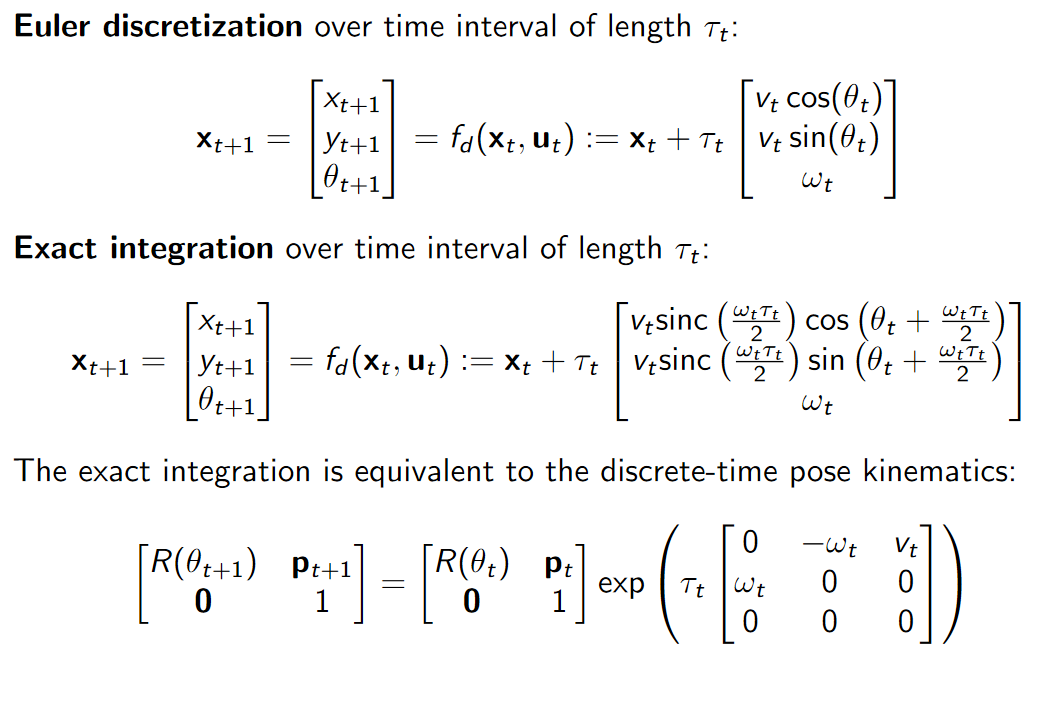
\includegraphics[width=12cm]{img/j_4_10.png}\end{figure}

The $sinc$ function is $\frac{\sin(x)}{x}$.